\section{Empirical Findings}
\label{sec:results}

We present results primarily through the German-English bilingual setup due to space constraints,  simulating the low-resource scenario with German.
Results for other languages and domains are consistent and discussed in Appendix~\ref{app:consistency}.

\paragraph{Data Repetition Leads to Predictable Overfitting}

Figure~\ref{fig:loss_curves} shows target-domain loss for the 143M model across three target dataset sizes, with each curve corresponding to a different target weight $h$. When $h$ forces high repetition, loss first improves then rises sharply, reflecting overfitting.
Target datasets of larger size delay this degradation because the same $h$ produces less repetition (Eq.~\ref{eq:main}).
Crucially, across all settings, overfitting onset is governed by the repetition factor $r$ alone: it means, the same target weight can be safe or harmful depending on the available dataset, but the same $r$ consistently triggers degradation regardless of how it is reached.               
This predictability of the same threshold, which holds across data sizes, model scales, and domains, motivates the scaling law in Section~\ref{sec:scaling_law}.

\paragraph{Mixture Training Unlocks High Repetition Tolerance}

Figure~\ref{fig:optimal_r} shows the optimal repetition factor (i.e., the value of $r$ that minimizes target loss) as a function of training tokens. 
Across all settings, optimal $r$ increases steadily with the training budget, reaching up to 15–20 depending on model size and dataset size, substantially exceeding the widely used rule-of-thumb of $<4$ epochs for single-source data-constrained training~\citep{muennighoff2023scaling}.
The difference stems from the generic domain, which provides a continuous supply of fresh tokens that effectively regularizes training and allows the model to absorb far more target-domain repetition before degradation sets in. Since $r$ results from the interplay of $h$, dataset size, and training budget (Eq.~\ref{eq:main}), the target weight needed to reach optimal $r$ varies widely, e.g., from 9.5\% (101M) to 1.9\% (539M) for the 50M dataset.


\begin{wrapfigure}{R}{0.52\textwidth}
\centering
\vspace{-15pt}
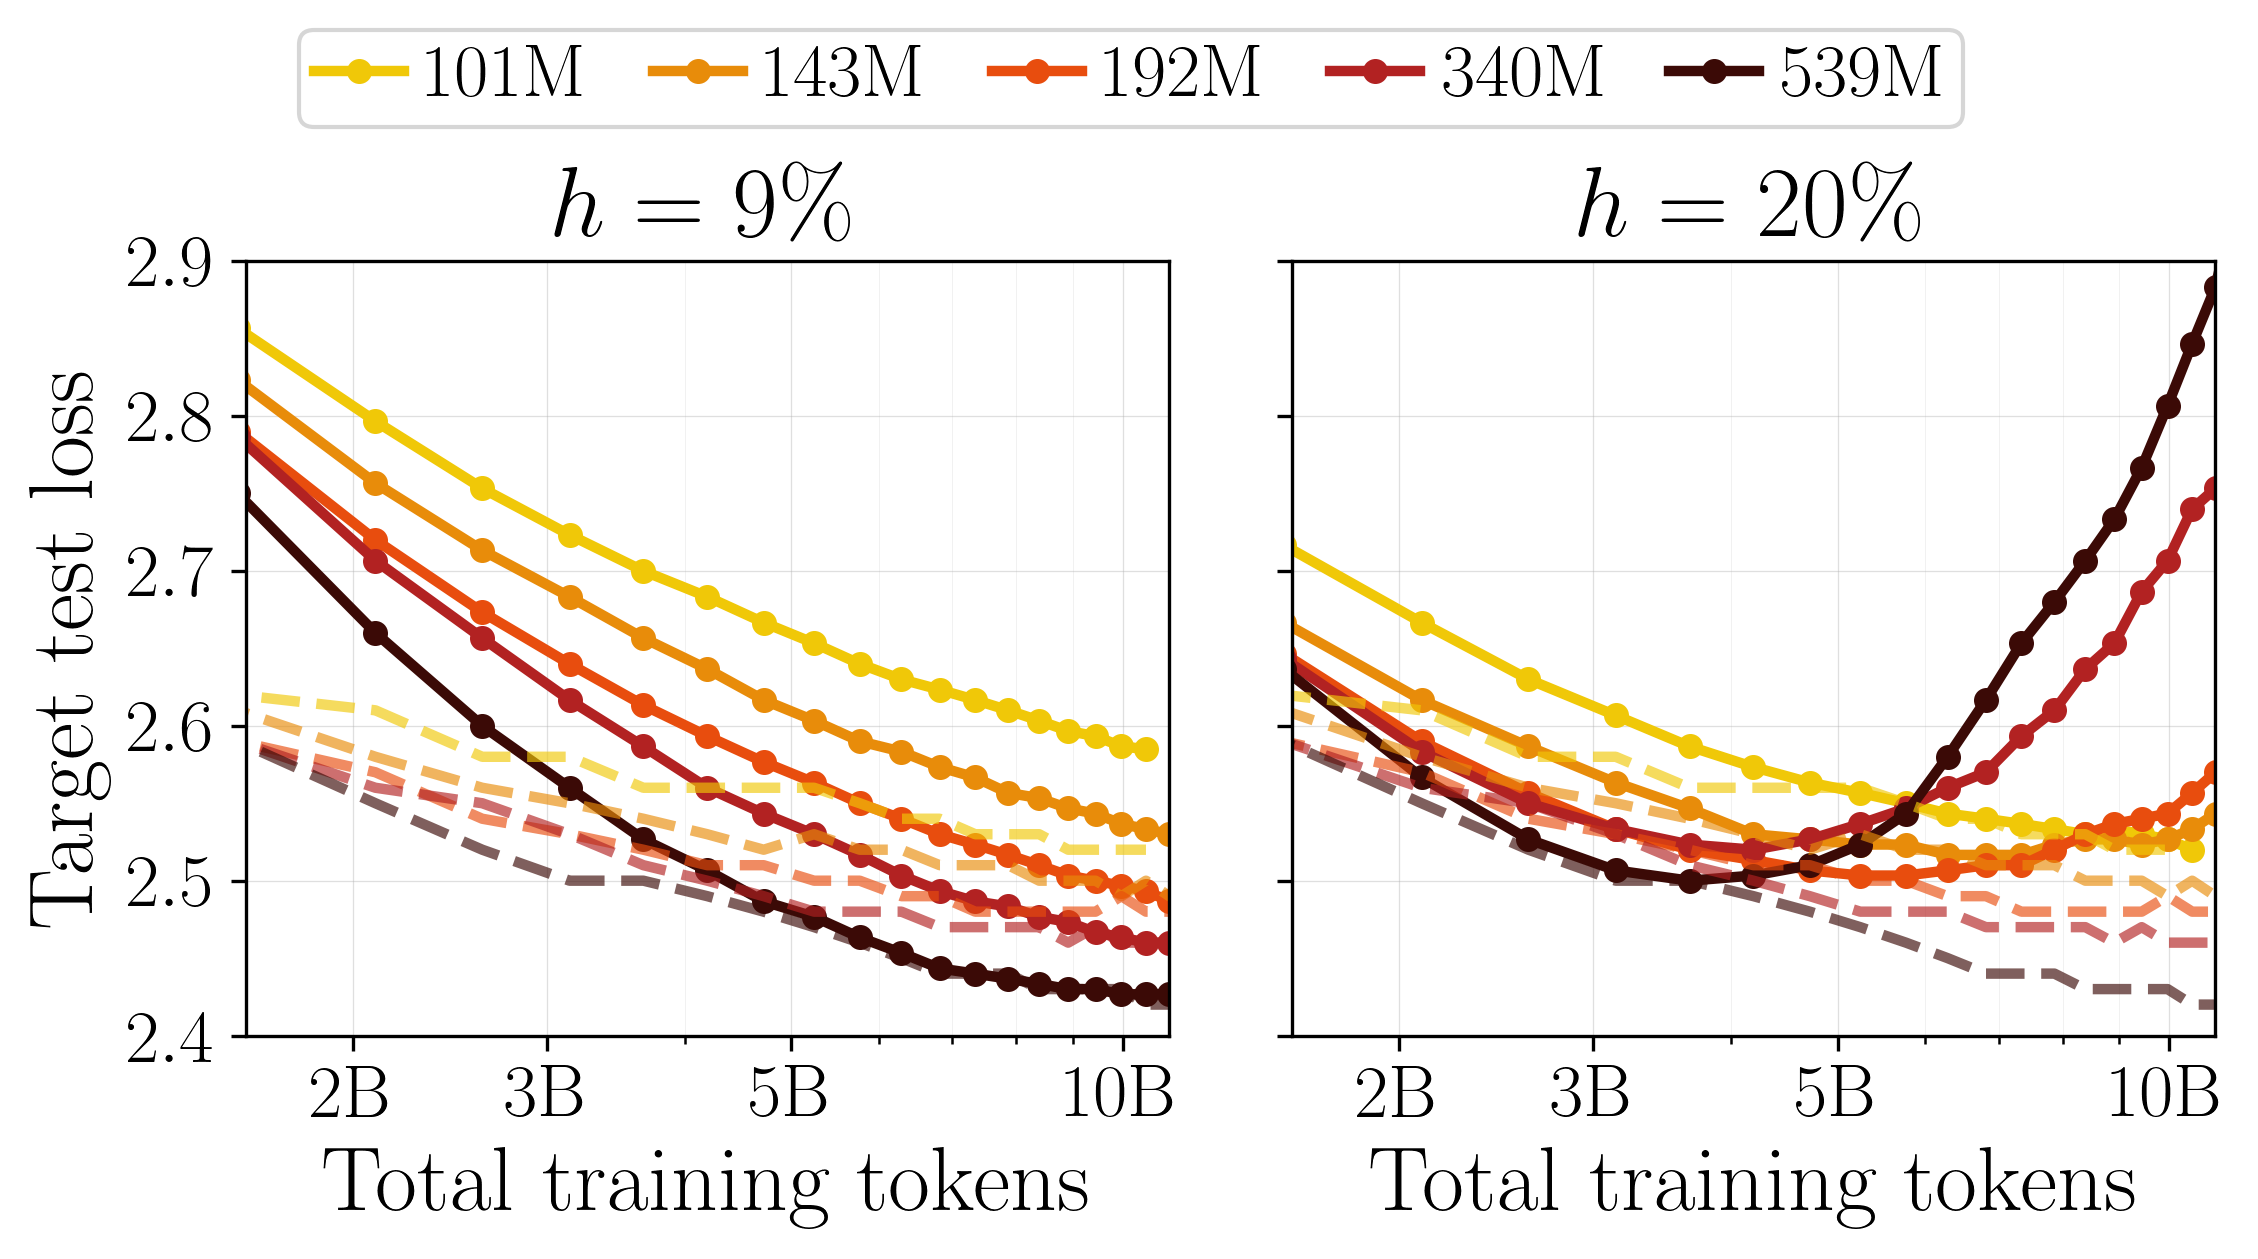
\includegraphics[width=0.52\textwidth]{figures/loss_curves_by_weight_de_100M_2panel.png}
\caption{Target-domain loss across model sizes at 9\% and 20\% target weights for fixed 100M German budget. Dashed lines show the best-loss envelope across all $h$ values. 
}
\label{fig:cross_model_fixed_h}
\vspace{-10pt}
\end{wrapfigure}

\paragraph{Larger Models Overfit Faster, Yet Still Win}
Figure~\ref{fig:cross_model_fixed_h} shows target-domain loss across five model sizes at two fixed target weights ($h = 9\%$ and $h = 20\%$) with 100M German tokens.
Dashed lines show the best-loss envelope, the minimum achievable loss at each training step across all $h$ values.
At $h = 9\%$, larger models plateau earlier while smaller models are still improving. At $h = 20\%$, the larger models eventually overfit (increasing target loss), while the smallest models plateau or still improve. 
This happens because larger models memorize the data more easily.
Yet in every case, larger models reach lower minima before degradation sets in, and the \emph{best-loss} envelope consistently favors larger models at every training budget.
Thus, we can conclude that \emph{scaling up remains beneficial} even under tight data constraints, but the optimal operating window narrows with model size. This also remains consistent with Figure~\ref{fig:optimal_r}, where the optimal repetition decreases with model size.

\begin{wrapfigure}{R}{0.4\textwidth}
\centering
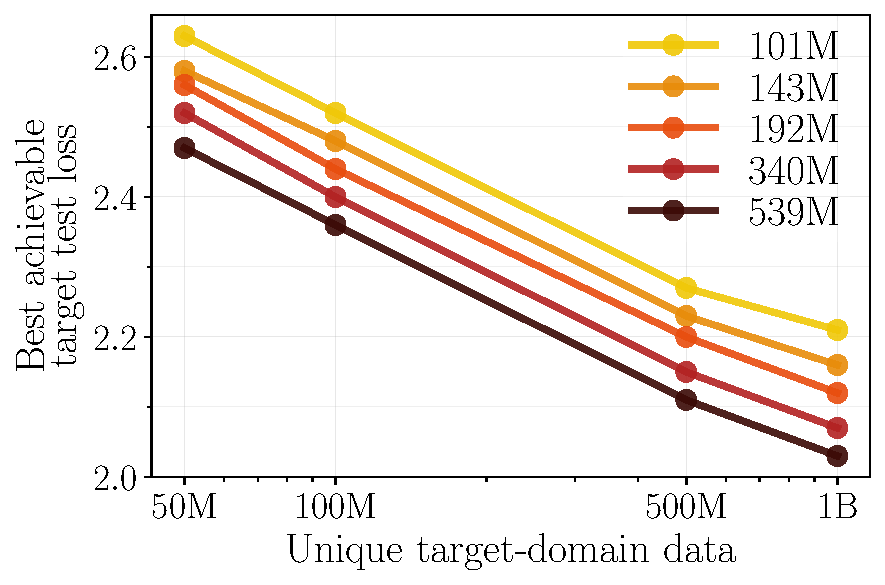
\includegraphics[width=0.4\textwidth]{figures/fig_diminishing_returns}
\vspace{-15pt}
\caption{Best achievable target loss by dataset size across different model sizes with optimal repetition.}
\vspace{-10pt}
\label{fig:diminishing}
\end{wrapfigure}
\paragraph{Predictable Scaling}
Figure~\ref{fig:diminishing} shows \emph{best} achievable loss as a function of unique data available among all weights $h$ and total training tokens, for different model sizes.
We see that these curves are remarkably regular: scaling up model size, or the number of available target data (e.g., by collecting fresh target data) both have a very predictable effect on the loss.

\paragraph{Broad Target Data Filters Can Beat More Repetitions}

The preceding experiments treat the domain dataset as fixed and study how repetition degrades loss. In some settings, however, the dataset size is a design choice as one can choose how to classify documents into the domain of interest. For example, using a quality filter at varying quality levels determines how much data remains, and a practitioner can trade quality for quantity by adjusting the threshold.  We use the Quality Data Mixture to determine whether accepting lower quality data (that is still data constrained and closer to the target domain) to reduce repetition yields better outcomes than repeating the highest quality data\footnote{For many data constrained domains, selecting the amount to filter out is tunable. We study data quality as existing work gives us an already established way of easily varying the amount of data and relevance to the target domain \citet{li2024datacomp}}.

To ground the experiment, we first confirm with a high quality target dataset of the 99th percentile and show loss curves at three dataset sizes (26M, 132M, 264M tokens) (see Figure~\ref{fig:top_1_data_constrained} in Appendix~\ref{app:quality_scales}). At the smallest scale, only $h \leq 0.1$ avoids overfitting, and larger sets progressively unlock higher sustainable target weights. This establishes the baseline that for a fixed quality threshold, the repetition penalty imposes the same constraint on the target loss.

\begin{wrapfigure}{r}{0.35\textwidth}
    \centering
    \vspace{-15pt}
    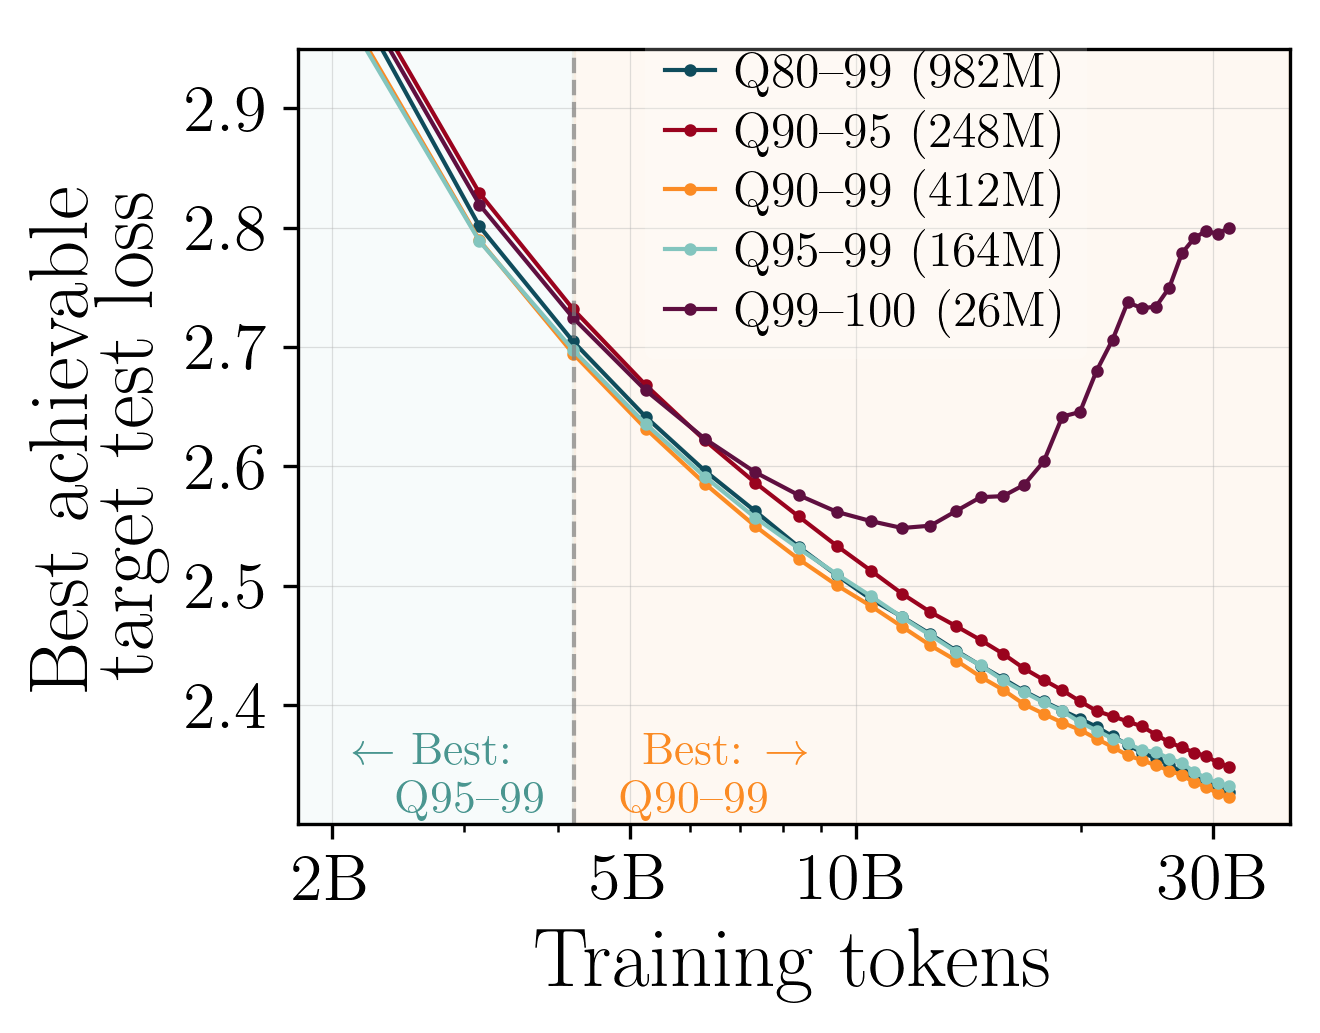
\includegraphics[width=0.35\textwidth]{figures/paper_comparison_02x_best_loss.png}
    \vspace{-20pt}
    \caption{Best loss by quality band. Dashed line marks the crossover where Q90-99 overtakes Q95-99.}
    \label{fig:comparison_best_loss}
    \vspace{-15pt}
\end{wrapfigure}
Next, we vary the quality filter threshold while holding the data source fixed. We fix the data constrained set such that the top 1\% (Q99-100) is 26M tokens, and add increasing amounts of data to the data constrained dataset at thresholds of 5\%, 10\%, and 20\% up to 982M tokens.  Results are in Figure~\ref{fig:comparison_combined}.  Relaxing the quality threshold and accepting slightly lower-quality data in exchange for a larger set consistently outperforms repeating a narrow high-quality slice. At Q99-100, only $h = 0.1$ avoids overfitting at up to 10B tokens of training, while Q90-99 supports weights up to $h = 0.4$ and Q80-99 shows nearly all weights monotonically decreasing.

\begin{figure}[t]
    \centering
    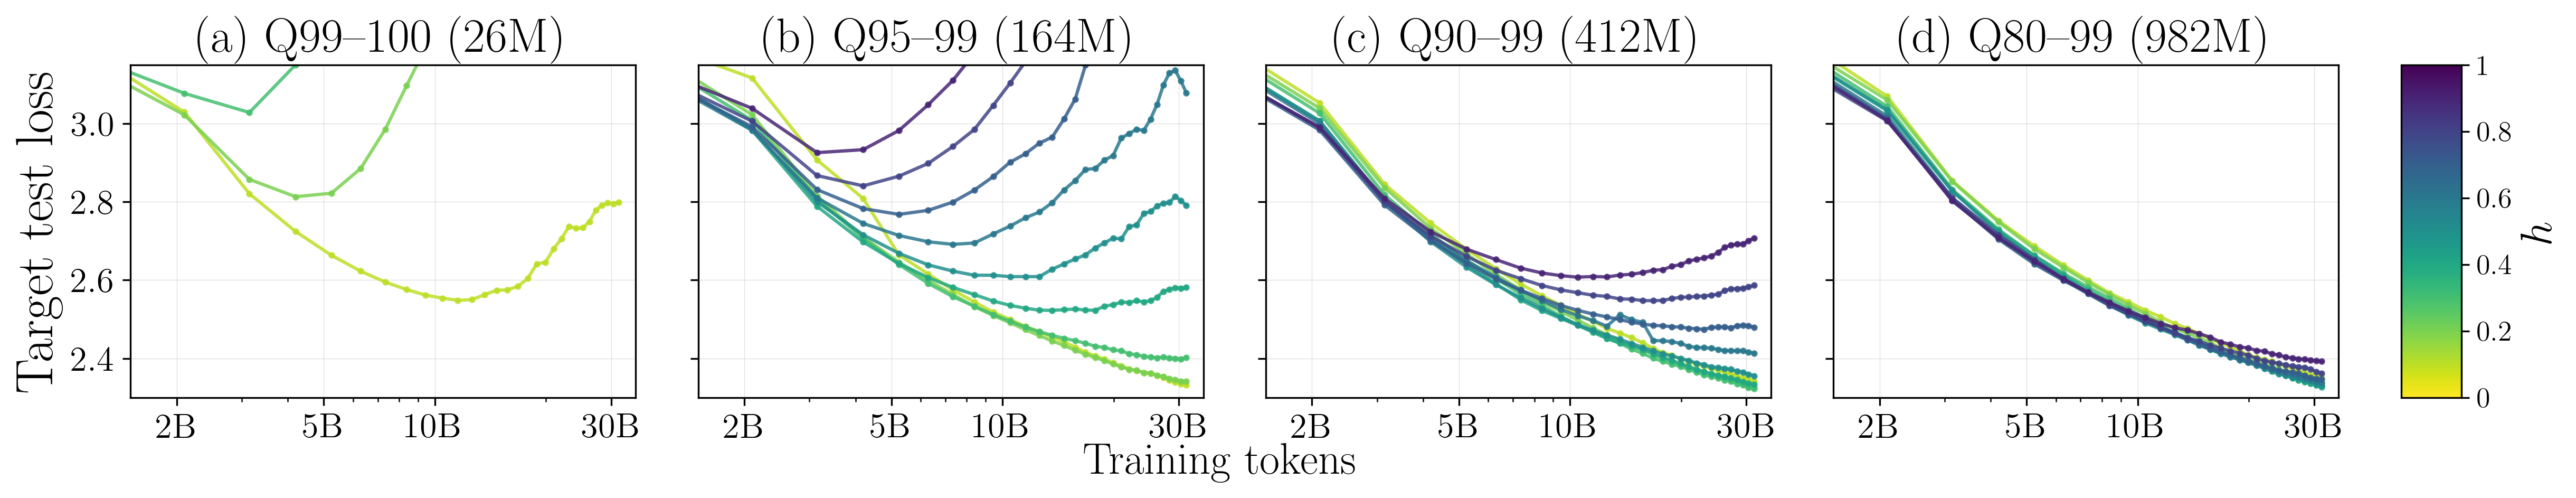
\includegraphics[width=\textwidth]{figures/paper_comparison_02x_combined.png}
    \caption{Loss curves for four quality bands ranging from 25M tokens at 99th percentile to 982M at the 80th, and ordered by increasing dataset size. Broader filters enable higher target weights without overfitting.}
    \label{fig:comparison_combined}
    \vspace{-5pt}
\end{figure}

The best quality set also depends on the training budget as we further observe that the best quality filter threshold changes at around 5B tokens as seen in Figure~\ref{fig:comparison_best_loss}, where the top 5\% high quality documents (Q95-99) performs best due to higher per-token quality, but the top 10\% set (Q90-99) overtakes it as training progresses and the smaller dataset saturates.
By 30B tokens, Q90-99 achieves loss 2.33 versus 2.80 for Q99-100 due to the repetition penalty.
This demonstrates that while repetition is an important factor, when high-quality data is scarce, broadening the filter is preferable to over repeating data.
